\section{Theorie}
\label{sec:Theorie}

Ziel des Versuchs ist es, das Elastizitätsmodul eines Metalls zu bestimmen und die berechneten Daten mit Literaturwerten abzugleichen.


\subsection{Allgemein}
In der Physik können Körper Gestalts- und Volumenänderungen erfahren, wenn Kräfte an der Oberfläche angreifen. Diese Kräfte werden Spannungskräfte genannt, welche sich auf Flächeneinheiten beziehen.
Die Spannung kann man komponentenweise aufteilen und die Komponente, die senkrecht zur Oberfläche steht, wird Normalspannung $\sigma$ oder Druck bezeichnet.
Tangential oder auch Schubspannung wird die oberflächenparalle Komponente genannt.
Die Gestaltsänderung kann beschrieben werden durch $\frac{\Delta L}{L}$. 
Ist diese hinreichend klein, kann ein linearer Zusammenhang zwischen der Deformation $\frac{\Delta L}{L}$ und der angreifenden Spannung $\sigma$ gebildet werden \cite[106]{V103}.  Das Hooksche Gesetz:
\begin{equation}
  \sigma = E \cdot \frac{\Delta L}{L}
  \label{eqn:Hook}
\end{equation}
E ist das Elastizitätsmodul, was eine materialabhängiger Proportionalitätsfaktor ist.
Dieses lässt sich bestimmen durch eine messbare Veränderung an einem Probestab bei nur geringer Krafteinwirkung. 
Diese Veränderung wird als Biegung bezeichnet, wobei die Durchbiegung $D(x)$ größer als $\frac{\Delta L}{L}$ ist bei gleichen Versuchbedingungen.


\subsection{einseitige Einspannung}

Wird der Stab einseitig eingespannt und auf der anderen Seite wirkt eine Kraft, entsteht eine Durchbiegung $D(x)$.
\begin{figure}
  \centering
  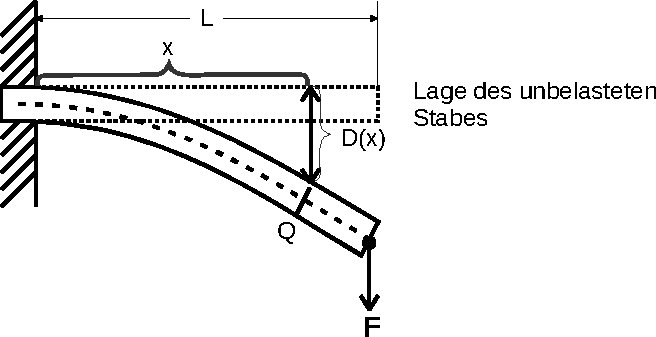
\includegraphics{content/einseitig.pdf}
  \caption{Durchbiegung eines elastischen Stabes bei einseitiger Einspannung \cite[107]{V103}}
  \label{fig:einseits}
\end{figure}
Entgegen der Kraft $F$ wirkt zusätzlich eine Zugspannung in der oberen Stabschicht und in der unteren eine Druckspannung (siehe \autoref{fig:einseits}) . 
Daraus lässt sich eine Drehmomentgleichung aufstellen:
\begin{equation}
    M_F = M_Q
\label{eqn:Drehgl}
\end{equation}
wobei das Drehmoment $M_Q$ sich aus der Integration über den Querschnitt $Q$ berechnet:
\begin{equation}
    M_Q = \int_Q y \sigma(y) dq.
    \label{eqn:M_Q}
\end{equation}
Das $y$ ist der Abstand zur neutralen Faser. Dies ist der Zustand ohne Spannung, also wenn keine Kräfte auf den Stab wirken.
Das Drehmoment $M_F$ ist die äußere Kraft, die auf den Stabquerschnitt an der Biegung $L-x$ angreift. 
Wobei $L$ die Länge des eingespannten Stabes ist.
\begin{equation}
    M_F = F(L-x)
    \label{eqn:M_F}
\end{equation}
Die beiden Drehmomente eingesetz in die Gleichung \autoref{eqn:Drehgl} ergeben:
\begin{equation}
  \int_Q y \sigma(y) dq = F(L-x).
\end{equation}
Durch Umformung der Gleichung und Beziehungen aus der Differentialgeometrie bei geringen Kurvenkrümmungen kann man des Hookschen Gesetzes für $\sigma(y)$ einsetzen:
\begin{equation}
   \sigma(y) = E y \frac{d^2D}{dx^2}.
\end{equation}
Außerdem kann das Flächenträgheitsmoment $I$ eingefügt werden, aufgrund der formalen Analogie zum Massenträgheitsmoment $\Theta$ \cite[109]{V103}.
\begin{equation}
   I = \int_Q y^2dq(y)
   \label{eqn:Flächenträgheitsmoment}
\end{equation}
Dies führt zur finalen Formel von $D(x)$ für die einseitige Einspannung:
\begin{equation}
  D(x) = \frac{F}{2 E I}(Lx^2 - \frac{x^3}{3}) \qquad (\text{für: } 0 \leq x \leq L)
  \label{eqn:Biegung}
\end{equation}

\subsection{beidseitige Auflage}

Eine andere Methode zur Erzeugung einer Durchbiegung ist es dein Stab auf beiden Seiten einzuspannen und ein Gewicht in die Mitte ein Gewicht zu hängen.
\begin{figure}[H]
  \centering
  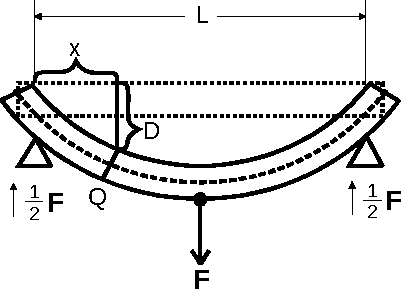
\includegraphics[height=4.5cm]{content/beidseits.pdf}
  \caption{Durchbiegung eines elastischen Stabes bei beidseitiger Auflage\cite[110]{V103}}
  \label{fig:beidseits}
\end{figure}
Dann greift die Kraft in der Mitte des Stabes an.
Am Querschnitt $Q$ mit dem Hebelarm $x$ beträgt die Kraft dann $\frac{F}{2}$ (siehe \autoref{fig:beidseits}). 
Deswegen muss der Stab in zwei Intervallen aufgeteilt werden, in denen sich das Drehmoment $M_F$ unterscheidet.\\
Im Bereich $ 0 \leq x \leq \frac{L}{2}$ gilt:
\begin{equation}
  M_F = -\frac{F}{2}x
  \label{eqn:M_F1}
\end{equation}
und in dem Bereich $\frac{F}{2} \leq x \leq L$ gilt:
\begin{equation}
  M_F = -\frac{F}{2}(L-x).
  \label{eqn:M_F2}
\end{equation}
Diese beiden Formeln werden beide in Gleichung \autoref{eqn:Drehgl} eingefügt und analog wie im vorherigen Kapitel umgeformt.
Sodass sich für $D(x)$ die folgenden Gleichungen ergeben:
\begin{align}
   D(x) = \frac{F}{48EI}(3L^2x - 4x^3) \qquad (\text{für: } 0 \leq x \leq \frac{L}{2})\label{eqn:Biegungbl}\\
   D(x) = \frac{F}{48EI}(4x^3 - 12Lx^2 + 9L^2x -L^3) \qquad (\text{für: } \frac{L}{2} \leq x \leq L)\label{eqn:Biegungbr}
\end{align}







